\documentclass[1p]{elsarticle_modified}
%\bibliographystyle{elsarticle-num}

%\usepackage[colorlinks]{hyperref}
%\usepackage{abbrmath_seonhwa} %\Abb, \Ascr, \Acal ,\Abf, \Afrak
\usepackage{amsfonts}
\usepackage{amssymb}
\usepackage{amsmath}
\usepackage{amsthm}
\usepackage{scalefnt}
\usepackage{amsbsy}
\usepackage{kotex}
\usepackage{caption}
\usepackage{subfig}
\usepackage{color}
\usepackage{graphicx}
\usepackage{xcolor} %% white, black, red, green, blue, cyan, magenta, yellow
\usepackage{float}
\usepackage{setspace}
\usepackage{hyperref}

\usepackage{tikz}
\usetikzlibrary{arrows}

\usepackage{multirow}
\usepackage{array} % fixed length table
\usepackage{hhline}

%%%%%%%%%%%%%%%%%%%%%
\makeatletter
\renewcommand*\env@matrix[1][\arraystretch]{%
	\edef\arraystretch{#1}%
	\hskip -\arraycolsep
	\let\@ifnextchar\new@ifnextchar
	\array{*\c@MaxMatrixCols c}}
\makeatother %https://tex.stackexchange.com/questions/14071/how-can-i-increase-the-line-spacing-in-a-matrix
%%%%%%%%%%%%%%%

\usepackage[normalem]{ulem}

\newcommand{\msout}[1]{\ifmmode\text{\sout{\ensuremath{#1}}}\else\sout{#1}\fi}
%SOURCE: \msout is \stkout macro in https://tex.stackexchange.com/questions/20609/strikeout-in-math-mode

\newcommand{\cancel}[1]{
	\ifmmode
	{\color{red}\msout{#1}}
	\else
	{\color{red}\sout{#1}}
	\fi
}

\newcommand{\add}[1]{
	{\color{blue}\uwave{#1}}
}

\newcommand{\replace}[2]{
	\ifmmode
	{\color{red}\msout{#1}}{\color{blue}\uwave{#2}}
	\else
	{\color{red}\sout{#1}}{\color{blue}\uwave{#2}}
	\fi
}

\newcommand{\Sol}{\mathcal{S}} %segment
\newcommand{\D}{D} %diagram
\newcommand{\A}{\mathcal{A}} %arc


%%%%%%%%%%%%%%%%%%%%%%%%%%%%%5 test

\def\sl{\operatorname{\textup{SL}}(2,\Cbb)}
\def\psl{\operatorname{\textup{PSL}}(2,\Cbb)}
\def\quan{\mkern 1mu \triangleright \mkern 1mu}

\theoremstyle{definition}
\newtheorem{thm}{Theorem}[section]
\newtheorem{prop}[thm]{Proposition}
\newtheorem{lem}[thm]{Lemma}
\newtheorem{ques}[thm]{Question}
\newtheorem{cor}[thm]{Corollary}
\newtheorem{defn}[thm]{Definition}
\newtheorem{exam}[thm]{Example}
\newtheorem{rmk}[thm]{Remark}
\newtheorem{alg}[thm]{Algorithm}

\newcommand{\I}{\sqrt{-1}}
\begin{document}

%\begin{frontmatter}
%
%\title{Boundary parabolic representations of knots up to 8 crossings}
%
%%% Group authors per affiliation:
%\author{Yunhi Cho} 
%\address{Department of Mathematics, University of Seoul, Seoul, Korea}
%\ead{yhcho@uos.ac.kr}
%
%
%\author{Seonhwa Kim} %\fnref{s_kim}}
%\address{Center for Geometry and Physics, Institute for Basic Science, Pohang, 37673, Korea}
%\ead{ryeona17@ibs.re.kr}
%
%\author{Hyuk Kim}
%\address{Department of Mathematical Sciences, Seoul National University, Seoul 08826, Korea}
%\ead{hyukkim@snu.ac.kr}
%
%\author{Seokbeom Yoon}
%\address{Department of Mathematical Sciences, Seoul National University, Seoul, 08826,  Korea}
%\ead{sbyoon15@snu.ac.kr}
%
%\begin{abstract}
%We find all boundary parabolic representation of knots up to 8 crossings.
%
%\end{abstract}
%\begin{keyword}
%    \MSC[2010] 57M25 
%\end{keyword}
%
%\end{frontmatter}

%\linenumbers
%\tableofcontents
%
\newcommand\colored[1]{\textcolor{white}{\rule[-0.35ex]{0.8em}{1.4ex}}\kern-0.8em\color{red} #1}%
%\newcommand\colored[1]{\textcolor{white}{ #1}\kern-2.17ex	\textcolor{white}{ #1}\kern-1.81ex	\textcolor{white}{ #1}\kern-2.15ex\color{red}#1	}

{\Large $\underline{12a_{0560}~(K12a_{0560})}$}

\setlength{\tabcolsep}{10pt}
\renewcommand{\arraystretch}{1.6}
\vspace{1cm}\begin{tabular}{m{100pt}>{\centering\arraybackslash}m{274pt}}
\multirow{5}{120pt}{
	\centering
	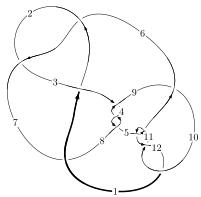
\includegraphics[width=112pt]{../../../GIT/diagram.site/Diagrams/png/1361_12a_0560.png}\\
\ \ \ A knot diagram\footnotemark}&
\allowdisplaybreaks
\textbf{Linearized knot diagam} \\
\cline{2-2}
 &
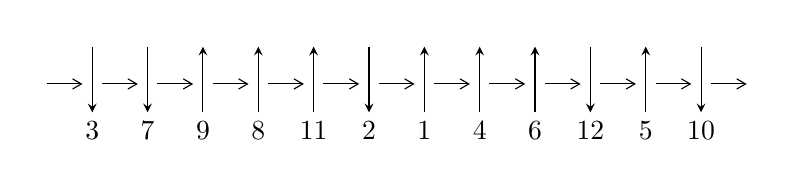
\begin{tikzpicture}[x=20pt, y=17pt]
	% nodes
	\node (C0) at (0, 0) {};
	\node (C1) at (1, 0) {};
	\node (C1U) at (1, +1) {};
	\node (C1D) at (1, -1) {3};

	\node (C2) at (2, 0) {};
	\node (C2U) at (2, +1) {};
	\node (C2D) at (2, -1) {7};

	\node (C3) at (3, 0) {};
	\node (C3U) at (3, +1) {};
	\node (C3D) at (3, -1) {9};

	\node (C4) at (4, 0) {};
	\node (C4U) at (4, +1) {};
	\node (C4D) at (4, -1) {8};

	\node (C5) at (5, 0) {};
	\node (C5U) at (5, +1) {};
	\node (C5D) at (5, -1) {11};

	\node (C6) at (6, 0) {};
	\node (C6U) at (6, +1) {};
	\node (C6D) at (6, -1) {2};

	\node (C7) at (7, 0) {};
	\node (C7U) at (7, +1) {};
	\node (C7D) at (7, -1) {1};

	\node (C8) at (8, 0) {};
	\node (C8U) at (8, +1) {};
	\node (C8D) at (8, -1) {4};

	\node (C9) at (9, 0) {};
	\node (C9U) at (9, +1) {};
	\node (C9D) at (9, -1) {6};

	\node (C10) at (10, 0) {};
	\node (C10U) at (10, +1) {};
	\node (C10D) at (10, -1) {12};

	\node (C11) at (11, 0) {};
	\node (C11U) at (11, +1) {};
	\node (C11D) at (11, -1) {5};

	\node (C12) at (12, 0) {};
	\node (C12U) at (12, +1) {};
	\node (C12D) at (12, -1) {10};
	\node (C13) at (13, 0) {};

	% arrows
	\draw[->,>={angle 60}]
	(C0) edge (C1) (C1) edge (C2) (C2) edge (C3) (C3) edge (C4) (C4) edge (C5) (C5) edge (C6) (C6) edge (C7) (C7) edge (C8) (C8) edge (C9) (C9) edge (C10) (C10) edge (C11) (C11) edge (C12) (C12) edge (C13) ;	\draw[->,>=stealth]
	(C1U) edge (C1D) (C2U) edge (C2D) (C3D) edge (C3U) (C4D) edge (C4U) (C5D) edge (C5U) (C6U) edge (C6D) (C7D) edge (C7U) (C8D) edge (C8U) (C9D) edge (C9U) (C10U) edge (C10D) (C11D) edge (C11U) (C12U) edge (C12D) ;
	\end{tikzpicture} \\
\hhline{~~} \\& 
\textbf{Solving Sequence} \\ \cline{2-2} 
 &
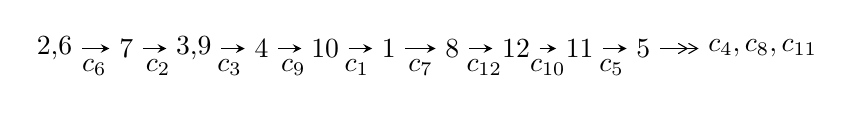
\begin{tikzpicture}[x=23pt, y=7pt]
	% node
	\node (A0) at (-1/8, 0) {2,6};
	\node (A1) at (1, 0) {7};
	\node (A2) at (33/16, 0) {3,9};
	\node (A3) at (25/8, 0) {4};
	\node (A4) at (33/8, 0) {10};
	\node (A5) at (41/8, 0) {1};
	\node (A6) at (49/8, 0) {8};
	\node (A7) at (57/8, 0) {12};
	\node (A8) at (65/8, 0) {11};
	\node (A9) at (73/8, 0) {5};
	\node (C1) at (1/2, -1) {$c_{6}$};
	\node (C2) at (3/2, -1) {$c_{2}$};
	\node (C3) at (21/8, -1) {$c_{3}$};
	\node (C4) at (29/8, -1) {$c_{9}$};
	\node (C5) at (37/8, -1) {$c_{1}$};
	\node (C6) at (45/8, -1) {$c_{7}$};
	\node (C7) at (53/8, -1) {$c_{12}$};
	\node (C8) at (61/8, -1) {$c_{10}$};
	\node (C9) at (69/8, -1) {$c_{5}$};
	\node (A10) at (11, 0) {$c_{4},c_{8},c_{11}$};

	% edge
	\draw[->,>=stealth]	
	(A0) edge (A1) (A1) edge (A2) (A2) edge (A3) (A3) edge (A4) (A4) edge (A5) (A5) edge (A6) (A6) edge (A7) (A7) edge (A8) (A8) edge (A9) ;
	\draw[->>,>={angle 60}]	
	(A9) edge (A10);
\end{tikzpicture} \\ 

\end{tabular} \\

\footnotetext{
The image of knot diagram is generated by the software ``\textbf{Draw programme}" developed by Andrew Bartholomew(\url{http://www.layer8.co.uk/maths/draw/index.htm\#Running-draw}), where we modified some parts for our purpose(\url{https://github.com/CATsTAILs/LinksPainter}).
}\phantom \\ \newline 
\centering \textbf{Ideals for irreducible components\footnotemark of $X_{\text{par}}$} 
 
\begin{align*}
I^u_{1}&=\langle 
1.46746\times10^{81} u^{97}-1.76536\times10^{81} u^{96}+\cdots+5.92140\times10^{81} b-1.09130\times10^{82},\\
\phantom{I^u_{1}}&\phantom{= \langle  }4.16618\times10^{81} u^{97}+1.31352\times10^{81} u^{96}+\cdots+5.92140\times10^{81} a+7.37637\times10^{81},\;u^{98}- u^{97}+\cdots- u+1\rangle \\
I^u_{2}&=\langle 
- u^2 a- u^2+b+a,\;u^3 a^2-3 a^2 u^2+2 u^3 a+a^3- a^2 u-5 u^2 a+u^3+3 a^2-2 u^2+2 a+u-1,\;u^4- u^2+1\rangle \\
\\
\end{align*}
\raggedright * 2 irreducible components of $\dim_{\mathbb{C}}=0$, with total 110 representations.\\
\footnotetext{All coefficients of polynomials are rational numbers. But the coefficients are sometimes approximated in decimal forms when there is not enough margin.}
\newpage
\renewcommand{\arraystretch}{1}
\centering \section*{I. $I^u_{1}= \langle 1.47\times10^{81} u^{97}-1.77\times10^{81} u^{96}+\cdots+5.92\times10^{81} b-1.09\times10^{82},\;4.17\times10^{81} u^{97}+1.31\times10^{81} u^{96}+\cdots+5.92\times10^{81} a+7.38\times10^{81},\;u^{98}- u^{97}+\cdots- u+1 \rangle$}
\flushleft \textbf{(i) Arc colorings}\\
\begin{tabular}{m{7pt} m{180pt} m{7pt} m{180pt} }
\flushright $a_{2}=$&$\begin{pmatrix}0\\u\end{pmatrix}$ \\
\flushright $a_{6}=$&$\begin{pmatrix}1\\0\end{pmatrix}$ \\
\flushright $a_{7}=$&$\begin{pmatrix}1\\u^2\end{pmatrix}$ \\
\flushright $a_{3}=$&$\begin{pmatrix}- u\\- u^3+u\end{pmatrix}$ \\
\flushright $a_{9}=$&$\begin{pmatrix}-0.703581 u^{97}-0.221826 u^{96}+\cdots+2.30148 u-1.24571\\-0.247823 u^{97}+0.298133 u^{96}+\cdots+0.142766 u+1.84297\end{pmatrix}$ \\
\flushright $a_{4}=$&$\begin{pmatrix}2.38586 u^{97}-2.00995 u^{96}+\cdots-3.05609 u-2.99728\\-1.02475 u^{97}+0.625222 u^{96}+\cdots-1.33955 u+0.977717\end{pmatrix}$ \\
\flushright $a_{10}=$&$\begin{pmatrix}-0.951404 u^{97}+0.0763073 u^{96}+\cdots+2.44424 u+0.597258\\-0.247823 u^{97}+0.298133 u^{96}+\cdots+0.142766 u+1.84297\end{pmatrix}$ \\
\flushright $a_{1}=$&$\begin{pmatrix}u^3\\u^5- u^3+u\end{pmatrix}$ \\
\flushright $a_{8}=$&$\begin{pmatrix}u^6- u^4+1\\u^8-2 u^6+2 u^4\end{pmatrix}$ \\
\flushright $a_{12}=$&$\begin{pmatrix}1.77227 u^{97}-1.68697 u^{96}+\cdots-6.38178 u-1.90346\\-0.845163 u^{97}+0.998105 u^{96}+\cdots-1.41033 u+0.784161\end{pmatrix}$ \\
\flushright $a_{11}=$&$\begin{pmatrix}0.474727 u^{97}+0.395086 u^{96}+\cdots+0.916706 u+0.647928\\0.354362 u^{97}-0.546426 u^{96}+\cdots+0.491807 u-1.27955\end{pmatrix}$ \\
\flushright $a_{5}=$&$\begin{pmatrix}1.65331 u^{97}-1.49550 u^{96}+\cdots-4.34761 u-2.09614\\-0.916624 u^{97}+0.581736 u^{96}+\cdots-0.992176 u+0.903994\end{pmatrix}$\\&\end{tabular}
\flushleft \textbf{(ii) Obstruction class $= -1$}\\~\\
\flushleft \textbf{(iii) Cusp Shapes $= 2.96382 u^{97}-1.51390 u^{96}+\cdots+0.841173 u-1.40563$}\\~\\
\newpage\renewcommand{\arraystretch}{1}
\flushleft \textbf{(iv) u-Polynomials at the component}\newline \\
\begin{tabular}{m{50pt}|m{274pt}}
Crossings & \hspace{64pt}u-Polynomials at each crossing \\
\hline $$\begin{aligned}c_{1}\end{aligned}$$&$\begin{aligned}
&u^{98}+49 u^{97}+\cdots+7 u+1
\end{aligned}$\\
\hline $$\begin{aligned}c_{2},c_{6}\end{aligned}$$&$\begin{aligned}
&u^{98}- u^{97}+\cdots- u+1
\end{aligned}$\\
\hline $$\begin{aligned}c_{3},c_{4},c_{8}\end{aligned}$$&$\begin{aligned}
&u^{98}- u^{97}+\cdots+85 u+25
\end{aligned}$\\
\hline $$\begin{aligned}c_{5},c_{11}\end{aligned}$$&$\begin{aligned}
&u^{98}+u^{97}+\cdots+7 u+1
\end{aligned}$\\
\hline $$\begin{aligned}c_{7}\end{aligned}$$&$\begin{aligned}
&u^{98}-3 u^{97}+\cdots-93143 u+31691
\end{aligned}$\\
\hline $$\begin{aligned}c_{9}\end{aligned}$$&$\begin{aligned}
&u^{98}-5 u^{97}+\cdots-30007 u+14539
\end{aligned}$\\
\hline $$\begin{aligned}c_{10},c_{12}\end{aligned}$$&$\begin{aligned}
&u^{98}+33 u^{97}+\cdots-9 u+1
\end{aligned}$\\
\hline
\end{tabular}\\~\\
\newpage\renewcommand{\arraystretch}{1}
\flushleft \textbf{(v) Riley Polynomials at the component}\newline \\
\begin{tabular}{m{50pt}|m{274pt}}
Crossings & \hspace{64pt}Riley Polynomials at each crossing \\
\hline $$\begin{aligned}c_{1}\end{aligned}$$&$\begin{aligned}
&y^{98}+7 y^{97}+\cdots+49 y+1
\end{aligned}$\\
\hline $$\begin{aligned}c_{2},c_{6}\end{aligned}$$&$\begin{aligned}
&y^{98}-49 y^{97}+\cdots-7 y+1
\end{aligned}$\\
\hline $$\begin{aligned}c_{3},c_{4},c_{8}\end{aligned}$$&$\begin{aligned}
&y^{98}+93 y^{97}+\cdots-20825 y+625
\end{aligned}$\\
\hline $$\begin{aligned}c_{5},c_{11}\end{aligned}$$&$\begin{aligned}
&y^{98}+33 y^{97}+\cdots-9 y+1
\end{aligned}$\\
\hline $$\begin{aligned}c_{7}\end{aligned}$$&$\begin{aligned}
&y^{98}+35 y^{97}+\cdots+1582314577 y+1004319481
\end{aligned}$\\
\hline $$\begin{aligned}c_{9}\end{aligned}$$&$\begin{aligned}
&y^{98}+21 y^{97}+\cdots-4470326109 y+211382521
\end{aligned}$\\
\hline $$\begin{aligned}c_{10},c_{12}\end{aligned}$$&$\begin{aligned}
&y^{98}+69 y^{97}+\cdots+27 y+1
\end{aligned}$\\
\hline
\end{tabular}\\~\\
\newpage\flushleft \textbf{(vi) Complex Volumes and Cusp Shapes}
$$\begin{array}{c|c|c}  
\text{Solutions to }I^u_{1}& \I (\text{vol} + \sqrt{-1}CS) & \text{Cusp shape}\\
 \hline 
\begin{aligned}
u &= -0.698281 + 0.734981 I \\
a &= -0.874615 - 0.965911 I \\
b &= \phantom{-}0.731025 + 0.877762 I\end{aligned}
 & \phantom{-}0.24752 + 2.82673 I & \phantom{-0.000000 } 0 \\ \hline\begin{aligned}
u &= -0.698281 - 0.734981 I \\
a &= -0.874615 + 0.965911 I \\
b &= \phantom{-}0.731025 - 0.877762 I\end{aligned}
 & \phantom{-}0.24752 - 2.82673 I & \phantom{-0.000000 } 0 \\ \hline\begin{aligned}
u &= -0.946641 + 0.419235 I \\
a &= \phantom{-}0.028820 - 0.209134 I \\
b &= \phantom{-}0.133572 - 0.403815 I\end{aligned}
 & -1.43448 + 1.60642 I & \phantom{-0.000000 } 0 \\ \hline\begin{aligned}
u &= -0.946641 - 0.419235 I \\
a &= \phantom{-}0.028820 + 0.209134 I \\
b &= \phantom{-}0.133572 + 0.403815 I\end{aligned}
 & -1.43448 - 1.60642 I & \phantom{-0.000000 } 0 \\ \hline\begin{aligned}
u &= \phantom{-}0.723311 + 0.768617 I \\
a &= -0.938705 + 1.015410 I \\
b &= \phantom{-}0.694302 - 1.112160 I\end{aligned}
 & -0.67700 - 8.24942 I & \phantom{-0.000000 } 0 \\ \hline\begin{aligned}
u &= \phantom{-}0.723311 - 0.768617 I \\
a &= -0.938705 - 1.015410 I \\
b &= \phantom{-}0.694302 + 1.112160 I\end{aligned}
 & -0.67700 + 8.24942 I & \phantom{-0.000000 } 0 \\ \hline\begin{aligned}
u &= -0.772111 + 0.515798 I \\
a &= -0.650090 - 0.932173 I \\
b &= \phantom{-}0.244840 + 0.118183 I\end{aligned}
 & -1.50656 + 2.09808 I & \phantom{-0.000000 } 0. - 4.26664 I \\ \hline\begin{aligned}
u &= -0.772111 - 0.515798 I \\
a &= -0.650090 + 0.932173 I \\
b &= \phantom{-}0.244840 - 0.118183 I\end{aligned}
 & -1.50656 - 2.09808 I & \phantom{-0.000000 -}0. + 4.26664 I \\ \hline\begin{aligned}
u &= \phantom{-}0.309981 + 0.864468 I \\
a &= -1.01439 - 1.42657 I \\
b &= \phantom{-}0.84080 + 1.59991 I\end{aligned}
 & -3.13766 + 11.40930 I & \phantom{-0.000000 } 0. - 6.77627 I \\ \hline\begin{aligned}
u &= \phantom{-}0.309981 - 0.864468 I \\
a &= -1.01439 + 1.42657 I \\
b &= \phantom{-}0.84080 - 1.59991 I\end{aligned}
 & -3.13766 - 11.40930 I & \phantom{-0.000000 -}0. + 6.77627 I\\
 \hline 
 \end{array}$$\newpage$$\begin{array}{c|c|c}  
\text{Solutions to }I^u_{1}& \I (\text{vol} + \sqrt{-1}CS) & \text{Cusp shape}\\
 \hline 
\begin{aligned}
u &= \phantom{-}1.038230 + 0.319222 I \\
a &= -1.226750 + 0.095271 I \\
b &= -0.232277 + 0.027239 I\end{aligned}
 & -1.83684 - 4.93742 I & \phantom{-0.000000 } 0 \\ \hline\begin{aligned}
u &= \phantom{-}1.038230 - 0.319222 I \\
a &= -1.226750 - 0.095271 I \\
b &= -0.232277 - 0.027239 I\end{aligned}
 & -1.83684 + 4.93742 I & \phantom{-0.000000 } 0 \\ \hline\begin{aligned}
u &= -0.933178 + 0.561155 I \\
a &= -0.19771 + 1.41969 I \\
b &= \phantom{-}1.271520 - 0.539820 I\end{aligned}
 & \phantom{-}3.33056 - 0.96432 I & \phantom{-0.000000 } 0 \\ \hline\begin{aligned}
u &= -0.933178 - 0.561155 I \\
a &= -0.19771 - 1.41969 I \\
b &= \phantom{-}1.271520 + 0.539820 I\end{aligned}
 & \phantom{-}3.33056 + 0.96432 I & \phantom{-0.000000 } 0 \\ \hline\begin{aligned}
u &= \phantom{-}0.815439 + 0.727212 I \\
a &= -0.81048 + 1.18357 I \\
b &= \phantom{-}0.085644 - 1.036660 I\end{aligned}
 & -5.05966 - 2.73854 I & \phantom{-0.000000 } 0 \\ \hline\begin{aligned}
u &= \phantom{-}0.815439 - 0.727212 I \\
a &= -0.81048 - 1.18357 I \\
b &= \phantom{-}0.085644 + 1.036660 I\end{aligned}
 & -5.05966 + 2.73854 I & \phantom{-0.000000 } 0 \\ \hline\begin{aligned}
u &= -1.070500 + 0.270114 I \\
a &= \phantom{-}0.968021 - 0.509743 I \\
b &= \phantom{-}0.457242 - 0.816853 I\end{aligned}
 & -0.736308 + 0.805438 I & \phantom{-0.000000 } 0 \\ \hline\begin{aligned}
u &= -1.070500 - 0.270114 I \\
a &= \phantom{-}0.968021 + 0.509743 I \\
b &= \phantom{-}0.457242 + 0.816853 I\end{aligned}
 & -0.736308 - 0.805438 I & \phantom{-0.000000 } 0 \\ \hline\begin{aligned}
u &= -0.647624 + 0.619058 I \\
a &= \phantom{-}1.59127 + 0.05416 I \\
b &= -1.167280 - 0.786021 I\end{aligned}
 & \phantom{-}4.16380 + 5.62077 I & \phantom{-}7.57068 - 6.82410 I \\ \hline\begin{aligned}
u &= -0.647624 - 0.619058 I \\
a &= \phantom{-}1.59127 - 0.05416 I \\
b &= -1.167280 + 0.786021 I\end{aligned}
 & \phantom{-}4.16380 - 5.62077 I & \phantom{-}7.57068 + 6.82410 I\\
 \hline 
 \end{array}$$\newpage$$\begin{array}{c|c|c}  
\text{Solutions to }I^u_{1}& \I (\text{vol} + \sqrt{-1}CS) & \text{Cusp shape}\\
 \hline 
\begin{aligned}
u &= -0.307950 + 0.837415 I \\
a &= -1.13129 + 1.41921 I \\
b &= \phantom{-}0.93785 - 1.45891 I\end{aligned}
 & -1.98077 - 5.63221 I & \phantom{-}2.48540 + 2.18051 I \\ \hline\begin{aligned}
u &= -0.307950 - 0.837415 I \\
a &= -1.13129 - 1.41921 I \\
b &= \phantom{-}0.93785 + 1.45891 I\end{aligned}
 & -1.98077 + 5.63221 I & \phantom{-}2.48540 - 2.18051 I \\ \hline\begin{aligned}
u &= \phantom{-}0.232349 + 0.855665 I \\
a &= -1.05558 - 1.08467 I \\
b &= \phantom{-}0.532748 + 1.218090 I\end{aligned}
 & -8.50104 + 5.18557 I & -4.36390 - 3.55063 I \\ \hline\begin{aligned}
u &= \phantom{-}0.232349 - 0.855665 I \\
a &= -1.05558 + 1.08467 I \\
b &= \phantom{-}0.532748 - 1.218090 I\end{aligned}
 & -8.50104 - 5.18557 I & -4.36390 + 3.55063 I \\ \hline\begin{aligned}
u &= \phantom{-}0.961002 + 0.564221 I \\
a &= -0.44703 - 1.38158 I \\
b &= \phantom{-}1.328800 + 0.254026 I\end{aligned}
 & \phantom{-}3.62769 - 4.71299 I & \phantom{-0.000000 } 0 \\ \hline\begin{aligned}
u &= \phantom{-}0.961002 - 0.564221 I \\
a &= -0.44703 + 1.38158 I \\
b &= \phantom{-}1.328800 - 0.254026 I\end{aligned}
 & \phantom{-}3.62769 + 4.71299 I & \phantom{-0.000000 } 0 \\ \hline\begin{aligned}
u &= \phantom{-}0.605300 + 0.626623 I \\
a &= \phantom{-}1.51979 + 0.06738 I \\
b &= -1.223730 + 0.519669 I\end{aligned}
 & \phantom{-}4.66705 + 0.02865 I & \phantom{-}8.77619 + 0.87832 I \\ \hline\begin{aligned}
u &= \phantom{-}0.605300 - 0.626623 I \\
a &= \phantom{-}1.51979 - 0.06738 I \\
b &= -1.223730 - 0.519669 I\end{aligned}
 & \phantom{-}4.66705 - 0.02865 I & \phantom{-}8.77619 - 0.87832 I \\ \hline\begin{aligned}
u &= -0.929226 + 0.670090 I \\
a &= -0.53068 - 1.33385 I \\
b &= -0.588519 + 0.613229 I\end{aligned}
 & -0.43509 + 2.50606 I & \phantom{-0.000000 } 0 \\ \hline\begin{aligned}
u &= -0.929226 - 0.670090 I \\
a &= -0.53068 + 1.33385 I \\
b &= -0.588519 - 0.613229 I\end{aligned}
 & -0.43509 - 2.50606 I & \phantom{-0.000000 } 0\\
 \hline 
 \end{array}$$\newpage$$\begin{array}{c|c|c}  
\text{Solutions to }I^u_{1}& \I (\text{vol} + \sqrt{-1}CS) & \text{Cusp shape}\\
 \hline 
\begin{aligned}
u &= \phantom{-}0.915941 + 0.711844 I \\
a &= -0.64807 + 1.38100 I \\
b &= -0.572020 - 0.910887 I\end{aligned}
 & -1.24817 + 2.69565 I & \phantom{-0.000000 } 0 \\ \hline\begin{aligned}
u &= \phantom{-}0.915941 - 0.711844 I \\
a &= -0.64807 - 1.38100 I \\
b &= -0.572020 + 0.910887 I\end{aligned}
 & -1.24817 - 2.69565 I & \phantom{-0.000000 } 0 \\ \hline\begin{aligned}
u &= \phantom{-}1.127030 + 0.285308 I \\
a &= \phantom{-}1.064220 + 0.673238 I \\
b &= \phantom{-}0.508509 + 1.058380 I\end{aligned}
 & -1.74262 + 4.42183 I & \phantom{-0.000000 } 0 \\ \hline\begin{aligned}
u &= \phantom{-}1.127030 - 0.285308 I \\
a &= \phantom{-}1.064220 - 0.673238 I \\
b &= \phantom{-}0.508509 - 1.058380 I\end{aligned}
 & -1.74262 - 4.42183 I & \phantom{-0.000000 } 0 \\ \hline\begin{aligned}
u &= \phantom{-}1.062130 + 0.488743 I \\
a &= -1.111330 - 0.750250 I \\
b &= \phantom{-}0.557998 - 0.549738 I\end{aligned}
 & -0.87096 - 4.56762 I & \phantom{-0.000000 } 0 \\ \hline\begin{aligned}
u &= \phantom{-}1.062130 - 0.488743 I \\
a &= -1.111330 + 0.750250 I \\
b &= \phantom{-}0.557998 + 0.549738 I\end{aligned}
 & -0.87096 + 4.56762 I & \phantom{-0.000000 } 0 \\ \hline\begin{aligned}
u &= \phantom{-}1.081070 + 0.447530 I \\
a &= \phantom{-}0.67659 + 1.70831 I \\
b &= -2.04138 - 0.47794 I\end{aligned}
 & -0.770537 - 0.474142 I & \phantom{-0.000000 } 0 \\ \hline\begin{aligned}
u &= \phantom{-}1.081070 - 0.447530 I \\
a &= \phantom{-}0.67659 - 1.70831 I \\
b &= -2.04138 + 0.47794 I\end{aligned}
 & -0.770537 + 0.474142 I & \phantom{-0.000000 } 0 \\ \hline\begin{aligned}
u &= \phantom{-}0.118232 + 0.819519 I \\
a &= -1.229960 - 0.561977 I \\
b &= \phantom{-}0.375994 + 0.574642 I\end{aligned}
 & -6.10324 - 1.41750 I & -2.21136 + 2.61331 I \\ \hline\begin{aligned}
u &= \phantom{-}0.118232 - 0.819519 I \\
a &= -1.229960 + 0.561977 I \\
b &= \phantom{-}0.375994 - 0.574642 I\end{aligned}
 & -6.10324 + 1.41750 I & -2.21136 - 2.61331 I\\
 \hline 
 \end{array}$$\newpage$$\begin{array}{c|c|c}  
\text{Solutions to }I^u_{1}& \I (\text{vol} + \sqrt{-1}CS) & \text{Cusp shape}\\
 \hline 
\begin{aligned}
u &= -1.107250 + 0.404686 I \\
a &= -1.38453 + 0.31849 I \\
b &= -0.137894 + 0.552380 I\end{aligned}
 & -2.25294 + 0.52462 I & \phantom{-0.000000 } 0 \\ \hline\begin{aligned}
u &= -1.107250 - 0.404686 I \\
a &= -1.38453 - 0.31849 I \\
b &= -0.137894 - 0.552380 I\end{aligned}
 & -2.25294 - 0.52462 I & \phantom{-0.000000 } 0 \\ \hline\begin{aligned}
u &= \phantom{-}1.115920 + 0.386738 I \\
a &= \phantom{-}0.770057 + 0.924879 I \\
b &= \phantom{-}0.001644 + 1.122350 I\end{aligned}
 & -5.78523 - 1.33156 I & \phantom{-0.000000 } 0 \\ \hline\begin{aligned}
u &= \phantom{-}1.115920 - 0.386738 I \\
a &= \phantom{-}0.770057 - 0.924879 I \\
b &= \phantom{-}0.001644 - 1.122350 I\end{aligned}
 & -5.78523 + 1.33156 I & \phantom{-0.000000 } 0 \\ \hline\begin{aligned}
u &= -1.075130 + 0.491781 I \\
a &= \phantom{-}0.321591 - 1.146720 I \\
b &= -0.529411 - 0.770162 I\end{aligned}
 & -0.78033 + 1.78897 I & \phantom{-0.000000 } 0 \\ \hline\begin{aligned}
u &= -1.075130 - 0.491781 I \\
a &= \phantom{-}0.321591 + 1.146720 I \\
b &= -0.529411 + 0.770162 I\end{aligned}
 & -0.78033 - 1.78897 I & \phantom{-0.000000 } 0 \\ \hline\begin{aligned}
u &= -1.086240 + 0.469331 I \\
a &= \phantom{-}1.00483 - 1.65568 I \\
b &= -2.08170 + 0.11796 I\end{aligned}
 & -0.60469 + 6.62618 I & \phantom{-0.000000 } 0 \\ \hline\begin{aligned}
u &= -1.086240 - 0.469331 I \\
a &= \phantom{-}1.00483 + 1.65568 I \\
b &= -2.08170 - 0.11796 I\end{aligned}
 & -0.60469 - 6.62618 I & \phantom{-0.000000 } 0 \\ \hline\begin{aligned}
u &= \phantom{-}0.800540 + 0.159505 I \\
a &= -1.34398 + 0.82795 I \\
b &= \phantom{-}0.235141 + 0.634144 I\end{aligned}
 & -3.78952 - 0.63574 I & -7.80030 - 1.07464 I \\ \hline\begin{aligned}
u &= \phantom{-}0.800540 - 0.159505 I \\
a &= -1.34398 - 0.82795 I \\
b &= \phantom{-}0.235141 - 0.634144 I\end{aligned}
 & -3.78952 + 0.63574 I & -7.80030 + 1.07464 I\\
 \hline 
 \end{array}$$\newpage$$\begin{array}{c|c|c}  
\text{Solutions to }I^u_{1}& \I (\text{vol} + \sqrt{-1}CS) & \text{Cusp shape}\\
 \hline 
\begin{aligned}
u &= -0.706846 + 0.404397 I \\
a &= \phantom{-}1.025440 + 0.209974 I \\
b &= -0.163790 - 0.549676 I\end{aligned}
 & -0.92183 + 1.73948 I & \phantom{-}1.33670 - 5.18470 I \\ \hline\begin{aligned}
u &= -0.706846 - 0.404397 I \\
a &= \phantom{-}1.025440 - 0.209974 I \\
b &= -0.163790 + 0.549676 I\end{aligned}
 & -0.92183 - 1.73948 I & \phantom{-}1.33670 + 5.18470 I \\ \hline\begin{aligned}
u &= -0.291710 + 0.746647 I \\
a &= \phantom{-}0.913446 - 0.553942 I \\
b &= -0.86158 + 1.20273 I\end{aligned}
 & \phantom{-}2.51136 - 7.38098 I & \phantom{-}4.67865 + 6.50498 I \\ \hline\begin{aligned}
u &= -0.291710 - 0.746647 I \\
a &= \phantom{-}0.913446 + 0.553942 I \\
b &= -0.86158 - 1.20273 I\end{aligned}
 & \phantom{-}2.51136 + 7.38098 I & \phantom{-}4.67865 - 6.50498 I \\ \hline\begin{aligned}
u &= -0.204099 + 0.770012 I \\
a &= -1.44727 + 0.96788 I \\
b &= \phantom{-}0.791296 - 0.812280 I\end{aligned}
 & -4.03937 - 2.88714 I & \phantom{-}1.97779 + 2.63363 I \\ \hline\begin{aligned}
u &= -0.204099 - 0.770012 I \\
a &= -1.44727 - 0.96788 I \\
b &= \phantom{-}0.791296 + 0.812280 I\end{aligned}
 & -4.03937 + 2.88714 I & \phantom{-}1.97779 - 2.63363 I \\ \hline\begin{aligned}
u &= \phantom{-}0.324606 + 0.719295 I \\
a &= \phantom{-}0.994278 + 0.499389 I \\
b &= -0.935589 - 0.987956 I\end{aligned}
 & \phantom{-}3.41838 + 1.78840 I & \phantom{-}6.81099 - 1.35188 I \\ \hline\begin{aligned}
u &= \phantom{-}0.324606 - 0.719295 I \\
a &= \phantom{-}0.994278 - 0.499389 I \\
b &= -0.935589 + 0.987956 I\end{aligned}
 & \phantom{-}3.41838 - 1.78840 I & \phantom{-}6.81099 + 1.35188 I \\ \hline\begin{aligned}
u &= \phantom{-}1.116840 + 0.479179 I \\
a &= \phantom{-}0.500971 + 1.225950 I \\
b &= -0.546443 + 1.046570 I\end{aligned}
 & -1.73593 - 7.03987 I & \phantom{-0.000000 } 0 \\ \hline\begin{aligned}
u &= \phantom{-}1.116840 - 0.479179 I \\
a &= \phantom{-}0.500971 - 1.225950 I \\
b &= -0.546443 - 1.046570 I\end{aligned}
 & -1.73593 + 7.03987 I & \phantom{-0.000000 } 0\\
 \hline 
 \end{array}$$\newpage$$\begin{array}{c|c|c}  
\text{Solutions to }I^u_{1}& \I (\text{vol} + \sqrt{-1}CS) & \text{Cusp shape}\\
 \hline 
\begin{aligned}
u &= \phantom{-}1.202550 + 0.232951 I \\
a &= -0.665302 - 0.130075 I \\
b &= -0.59992 - 1.56836 I\end{aligned}
 & -6.89377 + 2.42700 I & \phantom{-0.000000 } 0 \\ \hline\begin{aligned}
u &= \phantom{-}1.202550 - 0.232951 I \\
a &= -0.665302 + 0.130075 I \\
b &= -0.59992 + 1.56836 I\end{aligned}
 & -6.89377 - 2.42700 I & \phantom{-0.000000 } 0 \\ \hline\begin{aligned}
u &= \phantom{-}1.185840 + 0.328845 I \\
a &= -0.159149 + 0.253149 I \\
b &= -0.638766 - 1.188740 I\end{aligned}
 & -8.21277 - 0.66939 I & \phantom{-0.000000 } 0 \\ \hline\begin{aligned}
u &= \phantom{-}1.185840 - 0.328845 I \\
a &= -0.159149 - 0.253149 I \\
b &= -0.638766 + 1.188740 I\end{aligned}
 & -8.21277 + 0.66939 I & \phantom{-0.000000 } 0 \\ \hline\begin{aligned}
u &= -1.130920 + 0.495066 I \\
a &= -1.50190 + 0.76911 I \\
b &= \phantom{-}0.357862 + 1.110160 I\end{aligned}
 & -5.01226 + 6.39834 I & \phantom{-0.000000 } 0 \\ \hline\begin{aligned}
u &= -1.130920 - 0.495066 I \\
a &= -1.50190 - 0.76911 I \\
b &= \phantom{-}0.357862 - 1.110160 I\end{aligned}
 & -5.01226 - 6.39834 I & \phantom{-0.000000 } 0 \\ \hline\begin{aligned}
u &= \phantom{-}1.117680 + 0.547964 I \\
a &= -1.46662 - 1.06692 I \\
b &= \phantom{-}0.87922 - 1.22354 I\end{aligned}
 & \phantom{-}1.10367 - 6.62158 I & \phantom{-0.000000 } 0 \\ \hline\begin{aligned}
u &= \phantom{-}1.117680 - 0.547964 I \\
a &= -1.46662 + 1.06692 I \\
b &= \phantom{-}0.87922 + 1.22354 I\end{aligned}
 & \phantom{-}1.10367 + 6.62158 I & \phantom{-0.000000 } 0 \\ \hline\begin{aligned}
u &= -1.230070 + 0.222227 I \\
a &= -0.650623 + 0.287213 I \\
b &= -0.55993 + 1.63653 I\end{aligned}
 & -8.23592 - 8.08821 I & \phantom{-0.000000 } 0 \\ \hline\begin{aligned}
u &= -1.230070 - 0.222227 I \\
a &= -0.650623 - 0.287213 I \\
b &= -0.55993 - 1.63653 I\end{aligned}
 & -8.23592 + 8.08821 I & \phantom{-0.000000 } 0\\
 \hline 
 \end{array}$$\newpage$$\begin{array}{c|c|c}  
\text{Solutions to }I^u_{1}& \I (\text{vol} + \sqrt{-1}CS) & \text{Cusp shape}\\
 \hline 
\begin{aligned}
u &= -1.135920 + 0.548670 I \\
a &= -1.56765 + 1.05385 I \\
b &= \phantom{-}0.80759 + 1.40097 I\end{aligned}
 & \phantom{-}0.04166 + 12.27660 I & \phantom{-0.000000 } 0 \\ \hline\begin{aligned}
u &= -1.135920 - 0.548670 I \\
a &= -1.56765 - 1.05385 I \\
b &= \phantom{-}0.80759 - 1.40097 I\end{aligned}
 & \phantom{-}0.04166 - 12.27660 I & \phantom{-0.000000 } 0 \\ \hline\begin{aligned}
u &= -1.234570 + 0.289671 I \\
a &= -0.280220 + 0.162253 I \\
b &= -0.41036 + 1.42432 I\end{aligned}
 & -13.20240 - 1.48788 I & \phantom{-0.000000 } 0 \\ \hline\begin{aligned}
u &= -1.234570 - 0.289671 I \\
a &= -0.280220 - 0.162253 I \\
b &= -0.41036 - 1.42432 I\end{aligned}
 & -13.20240 + 1.48788 I & \phantom{-0.000000 } 0 \\ \hline\begin{aligned}
u &= -1.220590 + 0.363156 I \\
a &= \phantom{-}0.176181 - 0.092037 I \\
b &= -0.400866 + 0.960136 I\end{aligned}
 & -10.23010 + 5.45971 I & \phantom{-0.000000 } 0 \\ \hline\begin{aligned}
u &= -1.220590 - 0.363156 I \\
a &= \phantom{-}0.176181 + 0.092037 I \\
b &= -0.400866 - 0.960136 I\end{aligned}
 & -10.23010 - 5.45971 I & \phantom{-0.000000 } 0 \\ \hline\begin{aligned}
u &= -1.162350 + 0.529110 I \\
a &= \phantom{-}1.58602 - 0.69662 I \\
b &= -1.049770 - 0.884839 I\end{aligned}
 & -6.83271 + 7.72442 I & \phantom{-0.000000 } 0 \\ \hline\begin{aligned}
u &= -1.162350 - 0.529110 I \\
a &= \phantom{-}1.58602 + 0.69662 I \\
b &= -1.049770 + 0.884839 I\end{aligned}
 & -6.83271 - 7.72442 I & \phantom{-0.000000 } 0 \\ \hline\begin{aligned}
u &= \phantom{-}1.189490 + 0.501412 I \\
a &= \phantom{-}1.304510 + 0.485719 I \\
b &= -0.687871 + 0.503380 I\end{aligned}
 & -9.27708 - 3.36674 I & \phantom{-0.000000 } 0 \\ \hline\begin{aligned}
u &= \phantom{-}1.189490 - 0.501412 I \\
a &= \phantom{-}1.304510 - 0.485719 I \\
b &= -0.687871 - 0.503380 I\end{aligned}
 & -9.27708 + 3.36674 I & \phantom{-0.000000 } 0\\
 \hline 
 \end{array}$$\newpage$$\begin{array}{c|c|c}  
\text{Solutions to }I^u_{1}& \I (\text{vol} + \sqrt{-1}CS) & \text{Cusp shape}\\
 \hline 
\begin{aligned}
u &= -1.160770 + 0.580972 I \\
a &= \phantom{-}2.02321 - 0.58604 I \\
b &= -1.04158 - 1.61922 I\end{aligned}
 & -4.53003 + 10.88730 I & \phantom{-0.000000 } 0 \\ \hline\begin{aligned}
u &= -1.160770 - 0.580972 I \\
a &= \phantom{-}2.02321 + 0.58604 I \\
b &= -1.04158 + 1.61922 I\end{aligned}
 & -4.53003 - 10.88730 I & \phantom{-0.000000 } 0 \\ \hline\begin{aligned}
u &= \phantom{-}1.169640 + 0.590016 I \\
a &= \phantom{-}2.06628 + 0.49634 I \\
b &= -0.90929 + 1.73967 I\end{aligned}
 & -5.7221 - 16.7702 I & \phantom{-0.000000 } 0 \\ \hline\begin{aligned}
u &= \phantom{-}1.169640 - 0.590016 I \\
a &= \phantom{-}2.06628 - 0.49634 I \\
b &= -0.90929 - 1.73967 I\end{aligned}
 & -5.7221 + 16.7702 I & \phantom{-0.000000 } 0 \\ \hline\begin{aligned}
u &= \phantom{-}1.187170 + 0.556301 I \\
a &= \phantom{-}1.77127 + 0.43655 I \\
b &= -0.68854 + 1.25154 I\end{aligned}
 & -11.3632 - 10.3671 I & \phantom{-0.000000 } 0 \\ \hline\begin{aligned}
u &= \phantom{-}1.187170 - 0.556301 I \\
a &= \phantom{-}1.77127 - 0.43655 I \\
b &= -0.68854 - 1.25154 I\end{aligned}
 & -11.3632 + 10.3671 I & \phantom{-0.000000 } 0 \\ \hline\begin{aligned}
u &= -0.185731 + 0.641811 I \\
a &= \phantom{-}0.756552 - 0.283327 I \\
b &= -0.232991 + 0.941868 I\end{aligned}
 & -2.35932 - 2.00526 I & -1.48033 + 3.96035 I \\ \hline\begin{aligned}
u &= -0.185731 - 0.641811 I \\
a &= \phantom{-}0.756552 + 0.283327 I \\
b &= -0.232991 - 0.941868 I\end{aligned}
 & -2.35932 + 2.00526 I & -1.48033 - 3.96035 I \\ \hline\begin{aligned}
u &= \phantom{-}0.389023 + 0.509805 I \\
a &= \phantom{-}1.075130 + 0.144503 I \\
b &= -0.544827 - 0.221741 I\end{aligned}
 & \phantom{-}1.062250 + 0.424517 I & \phantom{-}8.97355 - 2.01331 I \\ \hline\begin{aligned}
u &= \phantom{-}0.389023 - 0.509805 I \\
a &= \phantom{-}1.075130 - 0.144503 I \\
b &= -0.544827 + 0.221741 I\end{aligned}
 & \phantom{-}1.062250 - 0.424517 I & \phantom{-}8.97355 + 2.01331 I\\
 \hline 
 \end{array}$$\newpage$$\begin{array}{c|c|c}  
\text{Solutions to }I^u_{1}& \I (\text{vol} + \sqrt{-1}CS) & \text{Cusp shape}\\
 \hline 
\begin{aligned}
u &= -0.290022 + 0.515209 I \\
a &= -0.018168 - 0.781517 I \\
b &= \phantom{-}0.879191 - 0.370054 I\end{aligned}
 & \phantom{-}1.36541 + 2.37978 I & \phantom{-}3.46852 - 3.41971 I \\ \hline\begin{aligned}
u &= -0.290022 - 0.515209 I \\
a &= -0.018168 + 0.781517 I \\
b &= \phantom{-}0.879191 + 0.370054 I\end{aligned}
 & \phantom{-}1.36541 - 2.37978 I & \phantom{-}3.46852 + 3.41971 I \\ \hline\begin{aligned}
u &= \phantom{-}0.127475 + 0.564967 I \\
a &= \phantom{-}0.312049 + 0.348058 I \\
b &= \phantom{-}0.714824 + 0.627954 I\end{aligned}
 & \phantom{-}0.89060 + 2.90592 I & \phantom{-}2.23821 - 2.15626 I \\ \hline\begin{aligned}
u &= \phantom{-}0.127475 - 0.564967 I \\
a &= \phantom{-}0.312049 - 0.348058 I \\
b &= \phantom{-}0.714824 - 0.627954 I\end{aligned}
 & \phantom{-}0.89060 - 2.90592 I & \phantom{-}2.23821 + 2.15626 I \\ \hline\begin{aligned}
u &= \phantom{-}0.445021 + 0.220782 I \\
a &= -2.67070 - 2.13843 I \\
b &= \phantom{-}1.43176 - 0.52942 I\end{aligned}
 & \phantom{-}1.36889 - 3.02323 I & \phantom{-}1.02541 + 1.50693 I \\ \hline\begin{aligned}
u &= \phantom{-}0.445021 - 0.220782 I \\
a &= -2.67070 + 2.13843 I \\
b &= \phantom{-}1.43176 + 0.52942 I\end{aligned}
 & \phantom{-}1.36889 + 3.02323 I & \phantom{-}1.02541 - 1.50693 I \\ \hline\begin{aligned}
u &= -0.334073 + 0.360832 I \\
a &= -2.92777 + 1.91022 I \\
b &= \phantom{-}1.54696 + 0.11678 I\end{aligned}
 & \phantom{-}1.58828 - 2.77548 I & \phantom{-}2.40050 + 3.94176 I \\ \hline\begin{aligned}
u &= -0.334073 - 0.360832 I \\
a &= -2.92777 - 1.91022 I \\
b &= \phantom{-}1.54696 - 0.11678 I\end{aligned}
 & \phantom{-}1.58828 + 2.77548 I & \phantom{-}2.40050 - 3.94176 I\\
 \hline 
 \end{array}$$\newpage\newpage\renewcommand{\arraystretch}{1}
\centering \section*{II. $I^u_{2}= \langle - u^2 a- u^2+b+a,\;u^3 a^2+2 u^3 a+\cdots+2 a-1,\;u^4- u^2+1 \rangle$}
\flushleft \textbf{(i) Arc colorings}\\
\begin{tabular}{m{7pt} m{180pt} m{7pt} m{180pt} }
\flushright $a_{2}=$&$\begin{pmatrix}0\\u\end{pmatrix}$ \\
\flushright $a_{6}=$&$\begin{pmatrix}1\\0\end{pmatrix}$ \\
\flushright $a_{7}=$&$\begin{pmatrix}1\\u^2\end{pmatrix}$ \\
\flushright $a_{3}=$&$\begin{pmatrix}- u\\- u^3+u\end{pmatrix}$ \\
\flushright $a_{9}=$&$\begin{pmatrix}a\\u^2 a+u^2- a\end{pmatrix}$ \\
\flushright $a_{4}=$&$\begin{pmatrix}u^3 a- u\\- a u\end{pmatrix}$ \\
\flushright $a_{10}=$&$\begin{pmatrix}u^2 a+u^2\\u^2 a+u^2- a\end{pmatrix}$ \\
\flushright $a_{1}=$&$\begin{pmatrix}u^3\\0\end{pmatrix}$ \\
\flushright $a_{8}=$&$\begin{pmatrix}- u^2+1\\u^2\end{pmatrix}$ \\
\flushright $a_{12}=$&$\begin{pmatrix}u^3 a^2+u^3 a+u^3+a u+u\\u^3 a^2+2 u^3 a- a^2 u+u\end{pmatrix}$ \\
\flushright $a_{11}=$&$\begin{pmatrix}u^3 a^2+2 u^2 a- u^3- a^2+2 a u+3 u^2-3 a+2 u-2\\u^3 a^2+2 u^3 a- a^2 u- u^2 a+u^3- u^2+a+u\end{pmatrix}$ \\
\flushright $a_{5}=$&$\begin{pmatrix}u^3 a\\u^3- a u- u\end{pmatrix}$\\&\end{tabular}
\flushleft \textbf{(ii) Obstruction class $= 1$}\\~\\
\flushleft \textbf{(iii) Cusp Shapes $= -4 a^2 u^2-4 u^3+4 a u+8 u^2-8 a+4 u-12$}\\~\\
\newpage\renewcommand{\arraystretch}{1}
\flushleft \textbf{(iv) u-Polynomials at the component}\newline \\
\begin{tabular}{m{50pt}|m{274pt}}
Crossings & \hspace{64pt}u-Polynomials at each crossing \\
\hline $$\begin{aligned}c_{1}\end{aligned}$$&$\begin{aligned}
&(u^2- u+1)^6
\end{aligned}$\\
\hline $$\begin{aligned}c_{2},c_{6},c_{7}\end{aligned}$$&$\begin{aligned}
&(u^4- u^2+1)^3
\end{aligned}$\\
\hline $$\begin{aligned}c_{3},c_{4},c_{8}\end{aligned}$$&$\begin{aligned}
&(u^2+1)^6
\end{aligned}$\\
\hline $$\begin{aligned}c_{5},c_{11}\end{aligned}$$&$\begin{aligned}
&(u^6+u^4+2 u^2+1)^2
\end{aligned}$\\
\hline $$\begin{aligned}c_{9}\end{aligned}$$&$\begin{aligned}
&(u^6-3 u^4+2 u^2+1)^2
\end{aligned}$\\
\hline $$\begin{aligned}c_{10}\end{aligned}$$&$\begin{aligned}
&(u^3- u^2+2 u-1)^4
\end{aligned}$\\
\hline $$\begin{aligned}c_{12}\end{aligned}$$&$\begin{aligned}
&(u^3+u^2+2 u+1)^4
\end{aligned}$\\
\hline
\end{tabular}\\~\\
\newpage\renewcommand{\arraystretch}{1}
\flushleft \textbf{(v) Riley Polynomials at the component}\newline \\
\begin{tabular}{m{50pt}|m{274pt}}
Crossings & \hspace{64pt}Riley Polynomials at each crossing \\
\hline $$\begin{aligned}c_{1}\end{aligned}$$&$\begin{aligned}
&(y^2+y+1)^6
\end{aligned}$\\
\hline $$\begin{aligned}c_{2},c_{6},c_{7}\end{aligned}$$&$\begin{aligned}
&(y^2- y+1)^6
\end{aligned}$\\
\hline $$\begin{aligned}c_{3},c_{4},c_{8}\end{aligned}$$&$\begin{aligned}
&(y+1)^{12}
\end{aligned}$\\
\hline $$\begin{aligned}c_{5},c_{11}\end{aligned}$$&$\begin{aligned}
&(y^3+y^2+2 y+1)^4
\end{aligned}$\\
\hline $$\begin{aligned}c_{9}\end{aligned}$$&$\begin{aligned}
&(y^3-3 y^2+2 y+1)^4
\end{aligned}$\\
\hline $$\begin{aligned}c_{10},c_{12}\end{aligned}$$&$\begin{aligned}
&(y^3+3 y^2+2 y-1)^4
\end{aligned}$\\
\hline
\end{tabular}\\~\\
\newpage\flushleft \textbf{(vi) Complex Volumes and Cusp Shapes}
$$\begin{array}{c|c|c}  
\text{Solutions to }I^u_{2}& \I (\text{vol} + \sqrt{-1}CS) & \text{Cusp shape}\\
 \hline 
\begin{aligned}
u &= \phantom{-}0.866025 + 0.500000 I \\
a &= -0.967306 - 0.373532 I \\
b &= \phantom{-}1.307140 + 0.215080 I\end{aligned}
 & \phantom{-}1.37919 + 0.79824 I & \phantom{-}1.50976 + 0.48465 I \\ \hline\begin{aligned}
u &= \phantom{-}0.866025 + 0.500000 I \\
a &= -0.006504 + 0.581105 I \\
b &= \phantom{-0.000000 -}0.569840 I\end{aligned}
 & -2.75839 - 2.02988 I & -5.01951 + 3.46410 I \\ \hline\begin{aligned}
u &= \phantom{-}0.866025 + 0.500000 I \\
a &= \phantom{-}0.33984 + 1.89050 I \\
b &= -1.307140 + 0.215080 I\end{aligned}
 & \phantom{-}1.37919 - 4.85801 I & \phantom{-}1.50976 + 6.44355 I \\ \hline\begin{aligned}
u &= \phantom{-}0.866025 - 0.500000 I \\
a &= -0.967306 + 0.373532 I \\
b &= \phantom{-}1.307140 - 0.215080 I\end{aligned}
 & \phantom{-}1.37919 - 0.79824 I & \phantom{-}1.50976 - 0.48465 I \\ \hline\begin{aligned}
u &= \phantom{-}0.866025 - 0.500000 I \\
a &= -0.006504 - 0.581105 I \\
b &= \phantom{-0.000000 } -0.569840 I\end{aligned}
 & -2.75839 + 2.02988 I & -5.01951 - 3.46410 I \\ \hline\begin{aligned}
u &= \phantom{-}0.866025 - 0.500000 I \\
a &= \phantom{-}0.33984 - 1.89050 I \\
b &= -1.307140 - 0.215080 I\end{aligned}
 & \phantom{-}1.37919 + 4.85801 I & \phantom{-}1.50976 - 6.44355 I \\ \hline\begin{aligned}
u &= -0.866025 + 0.500000 I \\
a &= -1.339840 + 0.158452 I \\
b &= \phantom{-}1.307140 + 0.215080 I\end{aligned}
 & \phantom{-}1.37919 + 4.85801 I & \phantom{-}1.50976 - 6.44355 I \\ \hline\begin{aligned}
u &= -0.866025 + 0.500000 I \\
a &= -0.99350 - 1.15095 I \\
b &= \phantom{-0.000000 -}0.569840 I\end{aligned}
 & -2.75839 + 2.02988 I & -5.01951 - 3.46410 I \\ \hline\begin{aligned}
u &= -0.866025 + 0.500000 I \\
a &= -0.03269 - 2.10558 I \\
b &= -1.307140 + 0.215080 I\end{aligned}
 & \phantom{-}1.37919 - 0.79824 I & \phantom{-}1.50976 - 0.48465 I \\ \hline\begin{aligned}
u &= -0.866025 - 0.500000 I \\
a &= -1.339840 - 0.158452 I \\
b &= \phantom{-}1.307140 - 0.215080 I\end{aligned}
 & \phantom{-}1.37919 - 4.85801 I & \phantom{-}1.50976 + 6.44355 I\\
 \hline 
 \end{array}$$\newpage$$\begin{array}{c|c|c}  
\text{Solutions to }I^u_{2}& \I (\text{vol} + \sqrt{-1}CS) & \text{Cusp shape}\\
 \hline 
\begin{aligned}
u &= -0.866025 - 0.500000 I \\
a &= -0.99350 + 1.15095 I \\
b &= \phantom{-0.000000 } -0.569840 I\end{aligned}
 & -2.75839 - 2.02988 I & -5.01951 + 3.46410 I \\ \hline\begin{aligned}
u &= -0.866025 - 0.500000 I \\
a &= -0.03269 + 2.10558 I \\
b &= -1.307140 - 0.215080 I\end{aligned}
 & \phantom{-}1.37919 + 0.79824 I & \phantom{-}1.50976 + 0.48465 I\\
 \hline 
 \end{array}$$\newpage
\newpage\renewcommand{\arraystretch}{1}
\centering \section*{ III. u-Polynomials}
\begin{tabular}{m{50pt}|m{274pt}}
Crossings & \hspace{64pt}u-Polynomials at each crossing \\
\hline $$\begin{aligned}c_{1}\end{aligned}$$&$\begin{aligned}
&((u^2- u+1)^6)(u^{98}+49 u^{97}+\cdots+7 u+1)
\end{aligned}$\\
\hline $$\begin{aligned}c_{2},c_{6}\end{aligned}$$&$\begin{aligned}
&((u^4- u^2+1)^3)(u^{98}- u^{97}+\cdots- u+1)
\end{aligned}$\\
\hline $$\begin{aligned}c_{3},c_{4},c_{8}\end{aligned}$$&$\begin{aligned}
&((u^2+1)^6)(u^{98}- u^{97}+\cdots+85 u+25)
\end{aligned}$\\
\hline $$\begin{aligned}c_{5},c_{11}\end{aligned}$$&$\begin{aligned}
&((u^6+u^4+2 u^2+1)^2)(u^{98}+u^{97}+\cdots+7 u+1)
\end{aligned}$\\
\hline $$\begin{aligned}c_{7}\end{aligned}$$&$\begin{aligned}
&((u^4- u^2+1)^3)(u^{98}-3 u^{97}+\cdots-93143 u+31691)
\end{aligned}$\\
\hline $$\begin{aligned}c_{9}\end{aligned}$$&$\begin{aligned}
&((u^6-3 u^4+2 u^2+1)^2)(u^{98}-5 u^{97}+\cdots-30007 u+14539)
\end{aligned}$\\
\hline $$\begin{aligned}c_{10}\end{aligned}$$&$\begin{aligned}
&((u^3- u^2+2 u-1)^4)(u^{98}+33 u^{97}+\cdots-9 u+1)
\end{aligned}$\\
\hline $$\begin{aligned}c_{12}\end{aligned}$$&$\begin{aligned}
&((u^3+u^2+2 u+1)^4)(u^{98}+33 u^{97}+\cdots-9 u+1)
\end{aligned}$\\
\hline
\end{tabular}\newpage\renewcommand{\arraystretch}{1}
\centering \section*{ IV. Riley Polynomials}
\begin{tabular}{m{50pt}|m{274pt}}
Crossings & \hspace{64pt}Riley Polynomials at each crossing \\
\hline $$\begin{aligned}c_{1}\end{aligned}$$&$\begin{aligned}
&((y^2+y+1)^6)(y^{98}+7 y^{97}+\cdots+49 y+1)
\end{aligned}$\\
\hline $$\begin{aligned}c_{2},c_{6}\end{aligned}$$&$\begin{aligned}
&((y^2- y+1)^6)(y^{98}-49 y^{97}+\cdots-7 y+1)
\end{aligned}$\\
\hline $$\begin{aligned}c_{3},c_{4},c_{8}\end{aligned}$$&$\begin{aligned}
&((y+1)^{12})(y^{98}+93 y^{97}+\cdots-20825 y+625)
\end{aligned}$\\
\hline $$\begin{aligned}c_{5},c_{11}\end{aligned}$$&$\begin{aligned}
&((y^3+y^2+2 y+1)^4)(y^{98}+33 y^{97}+\cdots-9 y+1)
\end{aligned}$\\
\hline $$\begin{aligned}c_{7}\end{aligned}$$&$\begin{aligned}
&((y^2- y+1)^6)(y^{98}+35 y^{97}+\cdots+1.58231\times10^{9} y+1.00432\times10^{9})
\end{aligned}$\\
\hline $$\begin{aligned}c_{9}\end{aligned}$$&$\begin{aligned}
&(y^3-3 y^2+2 y+1)^4\\
&\cdot(y^{98}+21 y^{97}+\cdots-4470326109 y+211382521)
\end{aligned}$\\
\hline $$\begin{aligned}c_{10},c_{12}\end{aligned}$$&$\begin{aligned}
&((y^3+3 y^2+2 y-1)^4)(y^{98}+69 y^{97}+\cdots+27 y+1)
\end{aligned}$\\
\hline
\end{tabular}
\vskip 2pc
\end{document}